% Chapter ComecocosWeb

\chapter{Comecocos Web} % Main chapter title
\section{Enunciado}
En esta práctica se pide elaborar un juego multimedia en primera persona. \\Actualmente existen varios juegos de este estilo por lo que el seleccionado es el clasico juego del Comecocos.La idea central del juego es manejar a Pacman por el escenario mientras huye de sus enemigos los fantamas.
\\A medida que Pacman se desplaza por el escenario va comiendo los cocos por lo que al comerselos todos el juego terminara.
\subsection*{Escenario}
El juego se lleva a cabo dentro del escenario del clasico juego de Pacman. Ademas de la pariencia del escenario se necesita generar los elementos basicos del mismo como son los obstaculos,los cocos, la casa de los fantasmas e informacion sobre la partida (puntuacion,vidas,cronometro)
\subsection*{Pacman}
Al ser un juego en primera persona es necesario crear un personaje principal (Pacman) que sera manejado por el usuario por el escenario.
\\Mientras Pacman se mueve interactuara con el escenario y sus elementos pero no podra sobrepasarlos por lo que se detendra al colisionar.Por ultimo,si la colision se produce con los enemigos Pacman pierde una vida y podria llegar a terminarse la partida.
\subsection*{Fantasmas}
Se tratan de los enemigos de Pacman en el juego.Al principio el unico fanstasma que se encuentra fuera de casa es 'blinky' el fantasma rojo quien inicia la persecucion de Pacman.A medida que la partida progresa los fantasmas restantes saldran para perseguir a Pacman.
\\El modo de persecucion de cada fantasma es autonomo entre cada uno y diferente.
\subsection{Tecnologias necesarias}
\begin{enumerate}
\item HTML5 tags : canvas,audio.
\item HTML5 API : LocalStorage
\item JavaScript
\end{enumerate}

\subsection{Objetivos}
\begin{enumerate}
\item Construir el juego con el interfaz grafico de HTML5.
\item Almacenamiento local del tiempo empleado para ganar la partida.
\item Implementar inteligencia Artificial 
\end{enumerate}
\section{Tecnologias aplicadas}
En este punto se explica los elementos que emplearemos de cada tecnologia en el desarrollo de esta practica.
\subsection{Canvas}
Se trata de una nueva etiqueta introducida en HTML5 que permite trabajar con graficos dentro de la web sin la necesidad de emplear programas externos.
A traves de los metodos de los que dispone permite relizar multiples tareas de caracter grafico de las cuales nosotros utilizaresmo las que se explican a continuacion..
\subsubsection*{Context 2d}
Es el punto de partida para utilizar las propiedades de canvas.Por ello se tiene que acceder a la etiqueta canvas existente en el documento lo que permite obtener el contexto.
En cuanto al contexto se utilizara el 2D ya que vamos a utilizar elemento planos aunque cabe destacar que es posible utilizar un contexto 3D.
\subsubsection*{Imagenes}
Esta propiedad nos permite manipular imagenes externas y presentarlas dentro de canvas.
Para ello diponemos del metodo 'context.drawImage()’ que se encuentra sobrecargado,es decir,segun el numero de parametros su funcionamiento varia.
\\En relacion a la practica se utilizan dos tipos de imagenes por lo que su tratamiento sera diferente a continuacion pasamos a explicar el enfoque dado en cada caso.
\begin{itemize}
\item Sprite sheet : imagen formada por pequeñas imagenes accesibles a traves de cortes en las dimensiones de cada elemento. Este comportamiento se realiza a traves del metodo 'drawImage(img,sx,sy,sw,sh,dx,dy,dw,dh)'que recibe como parametro la imagen,coordenadas y dimensiones de la imagen al igual que las coordenadas y dimensiones que este elemento ocupara dentro del canvas.
\begin{figure}[!h]
\begin{center}
   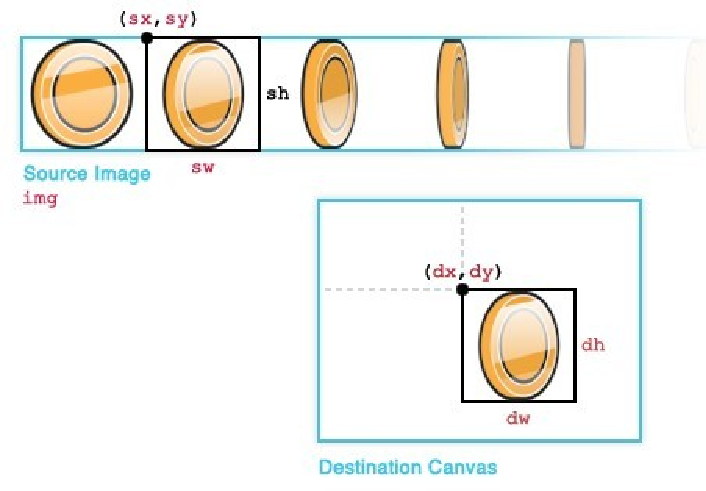
\includegraphics[width=0.4\linewidth]{Figures/SpreedSheet}
	\decoRule
	\caption[Contorno Escenario]{Contorno Escenario.}
\label{fig:canvasPrimitivas}
\end{center}
\end{figure}
\item Imagenes : a difertencia del caso anterior se carga la imagen completa a traves del metodo '.drawImage(img,0,0,canvas.width,canvas.height)' al que se le pasa la imagen y la coordenada y tamaño que la imagen ocupara en el canvas.
\end{itemize}
\subsubsection*{Texto}
Permite generar cadenas de texto dentro de canvas a traves del metodo 'fillText(text,x,y)' que recibe como parametro el texto y la coordenada donde se dibujara.En la practica se utiliza para mostrar la informacion del juego durante la partida.
\subsubsection*{Path}
Nos permite trabajar con un conjunto de  primitivas ya existente en canvas que son accesibles a traves del contexto.Dentro de ellas nosotros utilizamos las siguiente para dibujar los elementos del juego. 
\begin{itemize}
\item save()/restore(): metodos que permiten guardar el estado del dibujo y permite volver a obtener dicho estado.
\item beginPath() / closePath() : metodos que marcan el inicio y el final de los elementos que foman el dibujo que se necesite realizar.
\item moveTo(x,y): permite moverse a un punto del lienzo para empezar a dibujar a partir de el.
\item lineTo(x,y):a traves de este metodo podemos  dibujar una linea.Toma como punto de partida el ultimo punto conocido y como  punto final  la coordenada que se le pasa .
\item rect(x,y,width,heigth): permite dibujar un rectangulo con los parametro que se le pasa al metodo.
\item arc(x,y,radio,angInit,angFin,true): permite dibujar circunferencia,medias circunferenica. Para realizar este proceso establece como centro las coordenadas (x,y) ,su tamaño depende del radio que se especique y por ultimo establemos el angulo inical y final que queremos. 
\end{itemize}
\subsection{Inteligencia Artificial}
La inteligencia artificial permite simular el comportamiento de los personajes no manejados por el jugador:enemigos,animales.....
\\Se disponen de varias tecnicas que aplican este tipo comportamiento:
\begin{enumerate}
\item Minimax
\item Busqueda de caminos : A*
\item Maquina de estados finitos
\item Redes Neuronales
\item Redes evolutivas
\end{enumerate}
De las tecnicas anteriores la selecciona es la busqueda de caminos(A*) que se aplica a los fantasmas del juego para conseguir que persigan a Pacman de forma autonoma hasta capturarlo.
\\Esta tecnica necesita que el escenario se diseñe a traves de un grid(matriz bidimensional) que se convertira en el grafo de trabajo que permite calcular el camino mas corta entre un nodo inicial y un final.Cuando la busqueda  solo se tiene en cuenta los nodos transitables ya que el escenario del juego puede disponer de obstaculos.
\\Existen varios script que implementan esta tecnica como es el caso de 'astar.js' que sera el empleado en la practica.Para utilizarlo se necesita crear una matriz bidimensional con dos posibles valores el '0' que representa un obstaculo por lo que es un punto no accesible mientras que el valor '1' es un punto accesible.
\\A continuacion,se genera el grafo a traves de la funcion 'Grap(matriz)' y obtenemos el punto inicial y final mediante el metodo 'Graph.grid[x][y]' para cada uno de ellos. Finalmente obtenemos el camino mas corto entre los dos punto con el metodo 'search (pInicial, pFinal,false)‘.
 \begin{figure}[!h]
\begin{center}
   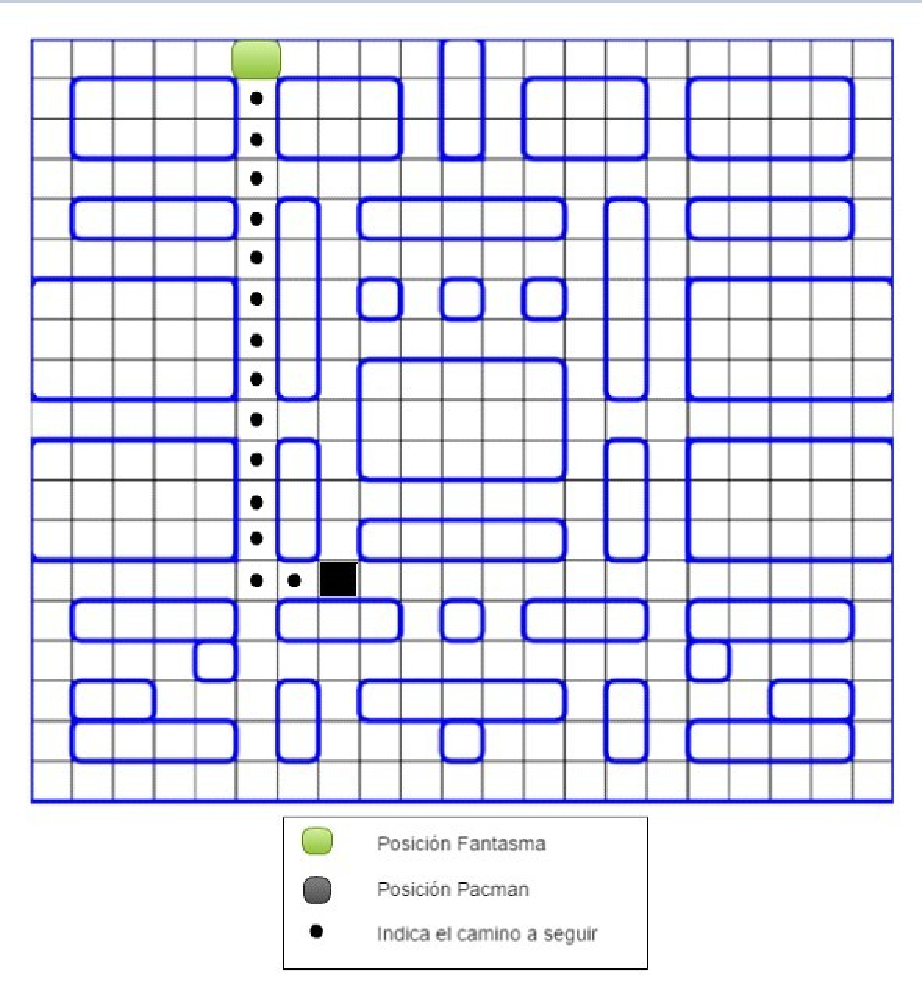
\includegraphics[width=0.6\linewidth, height=9cm]{Figures/InteligenciaArtificial}
	\decoRule
	\caption[Inteligencia Artificial]{Inteligencia Artificial.}
\label{fig:InteligenciaArtificial}
\end{center}
\end{figure}
\section{Esquema}
Se presenta un esquema de los puntos más importantes que nos podemos encontrarnos cuando se
ejecute el código. En cada momento se evalúa el comportamiento de Pacman ya actualizar sus
características depende de los elementos del entorno.
\begin{figure}[!h]
\centering
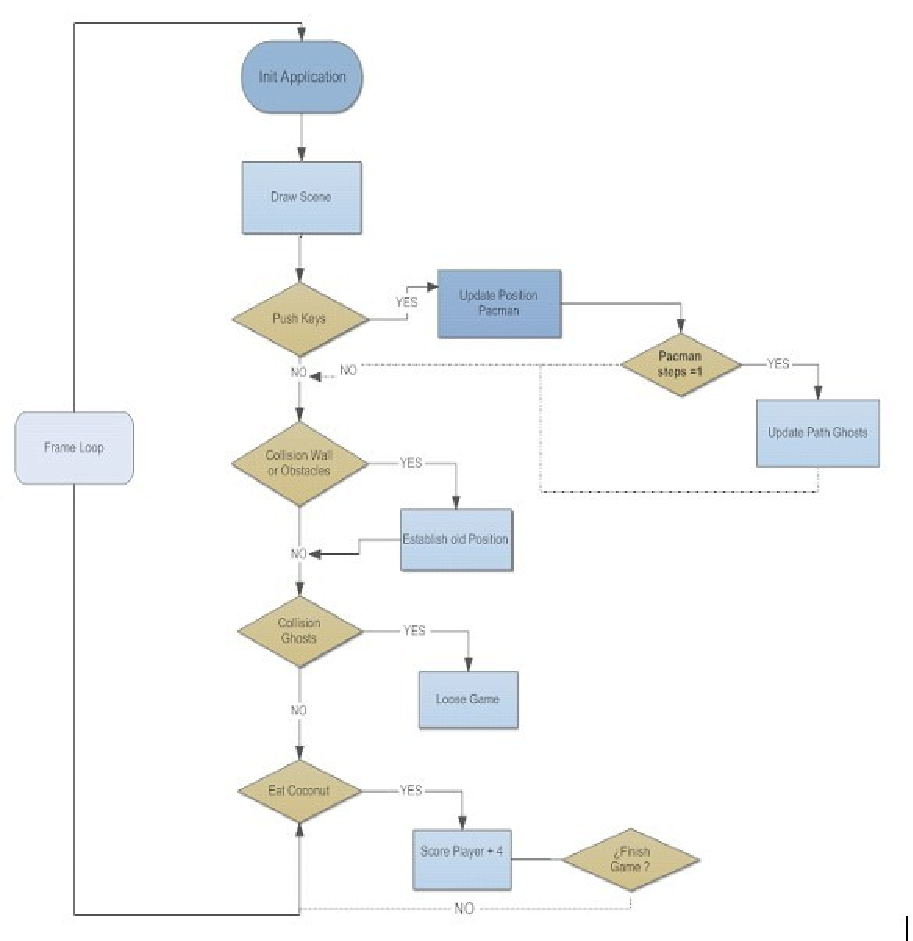
\includegraphics[width=0.8\linewidth]{Figures/esquemaP1}
\decoRule
\caption[Esquema funcional juego]{Esquema funcional del juego.}
\label{fig:esquemaP1}
\end{figure}
\section{Desarrollo}
Como se ha dicho a lo largo de este desarrollo la lógica del juego recae sobre JavaScript. Por esto se
han creado tres tipos de objetos (GameArea, Pacman, Ghost) con el objetivo de hacer más compacto
el código y menos repetitivo ya que hay muchas funciones que tienden a repetirse.
A continuación, explicaremos cada objeto la función que tienen en el juego.
\subsection{Game Area}
Este objeto es el encargado de generar y dibujar los elementos del  juego. Para realizar esto el objeto se inicializan una serie de variables al numero de filas y columnas de las que dispone del escenario y el tamaño de cada elemento. Ademas de los anteriores parametros se define la forma del escenario,obstaculos,cocos y la informacion de la partida.
\begin{lstlisting}[
frame=single,
commentstyle=\color{CadetBlue},
captionpos=b,
caption=Iniciacion de variables del Obj.Game]
  value_cuad : 40,
  filas:19,
  columnas:18,
  canvas : document.createElement("canvas"),
  image :new Image(),
  img_loose : new Image(),
  img_win : new Image(),
  /* time */
  seconds : 0,
  min : 0,
  horas :0,
  time : '00'+':'+'00'+':'+'00',
  /* state game */
  state : 0,
  score :0,
  start_crono : false,
  lifePlayer : 1,
  shape_1 : [...
  ],
  shape_2 : [...
  ],
  list_cocos : [...
  ],
  list_obstaculos : [...
  ],
\end{lstlisting}
Tras la definicion de las variables es necesario dotar al objeto de una serie de funciones que explicamos detalladamente a continuacion permitiendo dibujar el contenido del escenario.
\subsubsection*{Start}
Inicializa el tamaño del lienzo y genera el contexto de 'canvas' a traves del cual podremos dibujar el escenario y su contenido .Ademas,carga las imagenes y audios que se utilizaran en el juego.
\begin{lstlisting}[
frame=single,
commentstyle=\color{CadetBlue},
captionpos=b,
caption=Iniciacion de variables del Obj.Game]
 start : function() {
  this.img_loose.src ='game_over.jpeg';
  this.img_win.src = 'game_win.jpg';
  this.image.src = 'pacman_fruit.png';
  this.canvas.width = this.value_cuad*this.filas;
  this.canvas.height = this.value_cuad*(this.columnas+4);
  this.context = this.canvas.getContext("2d");
  document.body.insertBefore(this.canvas, 
  document.body.childNodes[2]);
  this.AudioGame =  document.getElementById('musica');
  this.AudioDied = document.getElementById('hitPacman');
  this.AudioEat = document.getElementById('eating');
 },
\end{lstlisting}
\subsubsection*{Escenario y elementos}
La creacion del escenario se realiza a traves de un array que contiene los comandos que se necesitan ejecutar para dibujar el contorno del escenario.
\begin{lstlisting}[
frame=single,
commentstyle=\color{CadetBlue},
captionpos=b,
caption=Visualizacion escenario.]
 shape_scene : function(shape){
  this.context.save();
  this.context.beginPath();
  for (var i = 0; i < shape.length; i++) {
   var elemento = shape[i];
   for (var propiedad in elemento){
    var x = elemento[propiedad];
    if(x.moveTo){
     this.context.moveTo(this.value_cuad*x.moveTo[0],
       this.value_cuad*x.moveTo[1]);
    }else if(x.lineTo){
     this.context.lineTo(x.lineTo[0]*this.value_cuad,
       this.value_cuad*x.lineTo[1]);
     }
    }
   }
   this.context.strokeStyle = 'blue';
   this.context.lineWidth = 2;
   this.context.stroke();
   this.context.restore();
   },
},
\end{lstlisting}
Los obstaculos del juego se dibujan a traves de la variable 'list\_obstaculos'.Cada elemento de esta variable esta formado por las coordenadas y dimensiones que se multiplican por el tamaño que tiene cada cuadro del escenario.
\begin{lstlisting}[
frame=single,
commentstyle=\color{CadetBlue},
captionpos=b,
caption= Visualizacion obstaculos.]
 draw_obstacles : function(){
   for(var i=0;i<this.list_obstaculos.length;i++){
    var elemento = this.list_obstaculos[i]; 
     this.context.fillRect(elemento.x*40,elemento.y*40,
       elemento.width*40,elemento.height*40);
   }
},
\end{lstlisting}
Los ultimos elementos del escenario son los cocos que sirven como comida a Pacman.Estos elementos se dibujan a traves de la variable 'list\_cocos' cuyo contenido sigue la misma logica que en los obstaculos.
\begin{lstlisting}[
frame=single,
commentstyle=\color{CadetBlue},
captionpos=b,
caption=Visualizacion cocos.]
 draw_doits : function(){
  if(this.list_cocos.length > 0){ 
   for(var i=0;i<this.list_cocos.length;i++){ 
    var elemento = this.list_cocos[i]; 
    this.context.fillStyle = 'white'; 
    this.context.beginPath(); 
    this.context.arc((elemento.x*40)+20,(elemento.y*40)+20,
       elemento.radio,0,(Math.PI/180),true);
    this.context.fill();
   }
 }
},
\end{lstlisting}
\subsubsection*{Informacion de la partida}
Se encarga de generar informacion para el usuario sobre el estado del juego a medida que la partida progresa.
\\Uno de los elementos es el cronometro que se dibuja mediante el metodo 'fillText()' que recibe como parametros la variable 'time' que se actualiza a traves de una funcion auxiliar que veremos mas adelante y la coordenada donde se quiere realizar el dibujo.
\begin{lstlisting}[
frame=single,
commentstyle=\color{CadetBlue},
captionpos=b,
caption=Visualizacion cronometro.]
 time_game:function(){
  this.context.save();
  this.context.font = "30px BDCartoonShoutRegular";	
  roundedRect(this.context,8*40,20*40,5*40,1*40,10);
  this.context.fillStyle = "#00FA9A";
  this.context.fillText(this.time,8.75*40,20.80*40);
  this.context.restore();
 },
 \end{lstlisting}
Tambien presenta la informacion del marcador del usuario a lo largo de la partida a traves de la varible 'score' que se actualizara a traves de una funcion auxuliar que veremos mas adelante.
\begin{lstlisting}[
frame=single,
commentstyle=\color{CadetBlue},
captionpos=b,
caption=Visualizacion Marcador.]
 score_user : function(){
  this.context.save();
  this.context.fillStyle = "white";
  this.context.font = "30px BDCartoonShoutRegular";
  this.context.fillText('score: '+this.score,1*40,20*40);
  this.context.restore();
 },
\end{lstlisting} 
Por ultimo muestra informacion del numero de vidas de las que dispone el usuario.El planteamiento aplicado es el mismo que en los casos anteriores aunque la varible 'life' vale siempre 1.
\begin{lstlisting}[
frame=single,
commentstyle=\color{CadetBlue},
captionpos=b,
caption=Visualizacion vidas.]
 life_user : function(){
  this.context.save();
  this.context.fillStyle = "white";
  this.context.font = "30px BDCartoonShoutRegular";
  this.context.fillText('life: '+this.life,1*40,21*40);
  this.context.restore();
 },
\end{lstlisting} 
\subsubsection*{Finalizacion Partida}
El ultimo punto a tratar del objeto es la generacion de contenido cuando termina la partida.
\\Puede terminar cuando Pacman ha logrado comerse todos los cocos de la partida dando lugar a la ejecucion de la funcion 'win\_game' la cual carga una imagen indicando al usuario que ha ganado y le permite guadar la informacion de la partida a traves de una funcion auxiliar que se explica mas adelante.
\begin{lstlisting}[
frame=single,
commentstyle=\color{CadetBlue},
captionpos=b,
caption=Visualizacion Partida Ganada.]
win_game : function(){
  var finish = false;
  if(this.list_cocos == 0){
    this.context.globalAlpha = 0.9;
    this.context.save();
    this.context.drawImage(this.img_win,0,0,
      this.canvas.width,this.canvas.height);
    roundedRect(this.context,this.canvas.width/2-(4*40),13*40,
      8*40,1.5*40,10);
    this.context.fillStyle = "#00FA9A";
    this.context.font = "30px BDCartoonShoutRegular";
    this.context.fillText('Save Score',
      this.canvas.width/2-(2.5*40),14*40);
    this.context.restore();
    finish = true;
   }
  return finish
},
\end{lstlisting} 
Otro forma en la que la patida termina es cuando los fantasmas capturan a Pacman dando lugar a la ejecucion de la funcion 'lose\_game' que carga una imagen indicando al usuario que ha perdido.
\begin{lstlisting}[
frame=single,
commentstyle=\color{CadetBlue},
captionpos=b,
caption=Visualizacion Partida Perdida.]
 lose_game : function(){
  this.context.save();
  this.context.globalAlpha = 0.6;	
  this.context.drawImage(this.img_loose,0,0,
    this.canvas.width,this.canvas.height);
  this.context.restore();
 },
\end{lstlisting} 
\subsection{Pacman}
Es el protagonista del juego y por ende el usuario interactúa con el moviéndolo por todo el
escenario. En su lógica tenemos que tener en cuenta diversos factores que afectan a su progreso
por el juego.
\subsubsection{Detectar colisiones}
Tenemos que tener en cuenta el entorno del juego con respecto a la posicion en la que se encuentra Pacman.Para ello la funcion 'hitt\_Counter' evalua que las coordena(x,y) no sobre pase el contorno del escenario.
 \begin{lstlisting}[
frame=single,
commentstyle=\color{CadetBlue},
captionpos=b,
caption=Deteccion de colisiones con el escenario.]
 this.hitt_counter = function(){
  var hitt_counter = false;
   if(this.x < 0 || this.x > GameArea.filas){
    hitt_counter = true;
   }else if(this.y < 0 || this.y > GameArea.columnas){
    hitt_counter = true;
   }
   return hitt_counter;
 }
 \end{lstlisting}
Otro punto importante es comprobar que la posicion de Pacman no sobrepase 
los objetos del juego. Para ello la funcion 'hitObject' recibe la lista de objetos de los que se quiere comprobar si existe colision con Pacman.
  \begin{lstlisting}[
frame=single,
commentstyle=\color{CadetBlue},
captionpos=b,
caption=Deteccion de colisiones con objetos del juego.]
 this.hitObject = function(list){
  var hitt = false;
  for(var i = 0;i<list.length;i++){
   var obstaculo = list[i];
   var Aobstaculo = {x:obstaculo.x,y:obstaculo.y};
   var Bobstaculo = {x:obstaculo.x+obstaculo.width,
       y:obstaculo.y};
   var Cobstaculo = {x:obstaculo.x,
       y:obstaculo.y+obstaculo.height};
   var Dobstaculo = {x:obstaculo.x+obstaculo.width,
       y:obstaculo.y+obstaculo.height};
   var Apac = {x:this.x,y:this.y};
   var Bpac = {x:this.x+this.width,y:this.y};
   var Cpac = {x:this.x,y:this.y+this.height};
   var Dpac = {x:this.x+this.width,y:this.y+this.height};
   if(Apac.x > Aobstaculo.x  && Apac.x < Bobstaculo.x &&
    Apac.y >  Aobstaculo.y && Apac.y < Cobstaculo.y){
    hitt = true;
    break
   }
   if(Bpac.x  >  Aobstaculo.x  && Bpac.x < Bobstaculo.x &&
    Bpac.y >  Aobstaculo.y && Bpac.y < Cobstaculo.y){
     hitt = true;
     break
   }
   if(Cpac.x >  Aobstaculo.x && Cpac.x < Bobstaculo.x && 
    Cpac.y >  Aobstaculo.y && Cpac.y < Cobstaculo.y){
     hitt = true;
     break
   }
   if(Dpac.x >   Aobstaculo.x && Dpac.x < Bobstaculo.x &&
    Dpac.y  >  Aobstaculo.y && Dpac.y <  Cobstaculo.y){
     hitt= true;
     break
   }
 }
 if(hitt == true){
  this.move = false;
 }
}
 \end{lstlisting}
\subsubsection{Comer Coco}
Los cocos se encuentran por el escenario por lo que es necesario comprobar  si hay colision ya que en caso de existir se actualiza el marcador del jugador y se elemina este elemento de la variable que contiene todos los cocos.
\begin{lstlisting}[
frame=single,
commentstyle=\color{CadetBlue},
captionpos=b,
caption=Deteccion de colision con los cocos.]
 this.eat_doit = function(list_cocos){
  var eat = false;
  for(var i=0;i<list_cocos.length;i++){
   var coco = list_cocos[i];
   var Apac = {x:this.x,y:this.y};
   var Bpac = {x:this.x+this.width,y:this.y};
   var Cpac = {x:this.x,y:this.y+this.height};
   var Dpac = {x:this.x+this.width,y:this.y+this.height};
    if (coco.x+0.5 > Apac.x && coco.x+0.5 < Bpac.x && 
      coco.y+0.5 > Apac.y && coco.y+0.5 < Cpac.y ){
      list_cocos.splice(i,1);
      eat = true
      GameArea.score = GameArea.score +4 ;
      break;
    }
   }
   return eat;
 }
 \end{lstlisting}
\subsubsection{Actualizar posicion Canvas}
Para actualizar las coordenadas de pacman correspondientes a su posicion actual se suma el numero de pasos dado al usuario realizar el movimiento a traves del teclado.
\begin{lstlisting}[
frame=single,
commentstyle=\color{CadetBlue},
captionpos=b,
caption=Actualizar posicion en canvas.]
 this.new_position = function (){
  this.x += this.speed_x;
  this.y += this.speed_y;
 }
 \end{lstlisting}
 Tras esto , actualizamos la variable 'pasos' que se utiliza para verificar cuando Pacman se ha desplazado a una nueva casilla del mapa del juego debido a que esta informacion es necesaria para aplicar IA. 
 \begin{lstlisting}[
 frame=single,
 commentstyle=\color{CadetBlue},
 captionpos=b,
 caption=Actualizacion de pasos dados]
 this.add_steps = function(){
  if(this.speed_x != 0 || this.speed_y != 0){
   if(this.type_move == 'y_pos' || this.type_move == "y_neg"){
    this.pasos += this.speed_y;
   }else{
    this.pasos += this.speed_x;
   }
  }
 }
\end{lstlisting}
\subsubsection{Actualizar posicion Mapa}
Actualizamos el valor de las variables 'x\_map' e 'y\_map' cuando la variable 'pasos' vale 1 ya que indica que se ha producido un desplzamiento completo a otra casilla. 
\begin{lstlisting}[
frame=single,
commentstyle=\color{CadetBlue},
captionpos=b,
caption=Actualizacion coordenada del mapa.]
 this.new_path = function(){
  if(this.x_map < 22 && this.x_map >= 0){
   if(this.y_map < 19 && this.y_map >= 0){
    if(this.type_move == 'y_pos'){
      this.y_map += 1;	
    }else if(this.type_move == 'x_pos'){
      this.x_map += 1;
	}else if(this.type_move == 'y_neg'){
      this.y_map -= 1;
    }else{
      this.x_map -= 1;
	}
    this.pasos = 0;
    this.new_pos = true;	
    }
  }
 }
 \end{lstlisting}
\subsubsection{Dibujar}
Finalmente,para dibujar a Pacman utilizamos la funcion 'drawImagen()' de canvas que cargam el trozo de imagen correspondiente a Pacman del spreedsheet.Posee dos estados de dibujo para crear la sensacion de animacion.
\begin{lstlisting}[
frame=single,
commentstyle=\color{CadetBlue},
captionpos=b,
caption=Dibujar Pacman.]
 this.draw = function(){
  GameArea.context.save();
  if(this.state_draw == 0){
   GameArea.context.drawImage(this.image,320,this.yDraw,32,32
     ,this.x*40,this.y*40,35,35);
   this.state_draw = 1;
  }else{
  GameArea.context.drawImage(this.image,320+32,this.yDraw,
      32,32,this.x*40,this.y*40,35,35);
    this.state_draw = 0;
  }
  GameArea.context.restore();
 }
 \end{lstlisting}
\subsection{Fantasmas}
Son los enemigos de Pacman que lo perseguirán por todo el escenario hasta que lo capturen. Son en total cuatro fantasmas con modos de persecución que varían entre si, por ello definimos un objeto llamado 'Ghost' con las funciones necesarias para generar su comportamiento.
\subsubsection{Actualizar objetivo}
Esta funcion se encarga de aplicar  IA en cada uno de los fantasmas ya que como se explico en la seccion 'Tecnologias aplicadas' de esta practica a traves del mapa del juego obtemos el camino que cada fantasma tiene que seguir. Para ello tomamos como punto de inicio la posicion actual del fantasma y la posicion de Pacman formado por las variables 'x map' e 'y map' como punto de destino.
\\A continuacion explicamos el modo de busqueda que los fantasmas utilizan para llegar a Pacman.
\begin{itemize}
\item \textit{Blinky}: haciendo referencia a la historia del juego, el comportamiento del fantasma es seguir a Pacman en la misma dirección, entonces el punto de inicio es la posición actual de fantasma y el punto final es la nueva posición de Pacman.
\item \textit{Speedy}:al igual que Blinky su comportamiento es seguir a Pacman, pero tiene en cuenta la dirección en la que Pacman se mueve. En este caso el cálculo se realiza como punto de
partida la posición de Speedy y se consulta la dirección de Pacman y le sumamos/ restamos 4 posiciones según corresponda para obtener el punto final.
\item \textit{Clyde}:tiene dos tipos de comportamientos que dependen de la distancia entre él y Pacman, si dicha distancia es mayor a ocho sigue en modo persecución en caso contrario deja de seguirlo y se aleja de él tomando como objetivo nuevo una de las esquinas
\end{itemize}
\begin{lstlisting}[
frame=single,
commentstyle=\color{CadetBlue},
captionpos=b,
caption=.Actualizar direccion hacia el objetivo]
 this.new_path = function(graph,pacman_x,pacman_y,direccion){
  var start = graph.grid[this.x_map][this.y_map];
  if(this.name == 'blinky'){
   var end = graph.grid[pacman_x][pacman_y];
  }else if(this.name == 'speedy'){
   if(pacman_x+4 < 21 && direccion == 'x_pos'){
    pacman_x += 4;
   }else if(pacman_x-4 > 0 && direccion == 'x_neg'){
    pacman_x -= 4;
   }else if(pacman_y+4 < 19 && direccion == 'y_pos'){
    pacman_y += 4;
   }else if(pacman_y-4 > 0 && direccion == 'y_neg'){
    pacman_y -= 4;
   }
   var end = graph.grid[pacman_x][pacman_y];
  }else if (this.name == 'clyde'){
   var end = graph.grid[pacman_x][pacman_y];
   this.result = astar.search(graph,start,end,false);
   if(this.result.length < 8){
   var end = graph.grid[this.cuad_static.x][this.cuad_static.y];
   }
  }
  this.result = astar.search(graph,start,end,false);
 }
\end{lstlisting}
\subsubsection{Actualizar posición}
Una vez se obtiene el camino que cada fantasma tiene que seguir para intentar capturar al objetivo se actualiza la posicion de cada fantasma a traves de un evento timer que se ejecuta segun el valor definido en la variable speed de cada uno.
\\En el momento de la ejecucion se actualiza la posicion del fantamas con la informacion del siguiente punto del camino que posee cada fantasma.
\begin{lstlisting}[
frame=single,
commentstyle=\color{CadetBlue},
captionpos=b,
caption=Actualizar posicion del los Fantasmas.]
 function nexStepGhost(ghost){
 ghost.flag = 1;
 if(ghost.result.length > 0){
  ghost.x = ghost.result[0].x;
  ghost.y = ghost.result[0].y;
  ghost.x_map = ghost.result[0].x;
  ghost.y_map = ghost.result[0].y;
  ghost.result.splice(0,1);
 }
 ghost.interval = setTimeout(function(){
  nexStepGhost(ghost)
  },ghost.speed);
 }
\end{lstlisting}
\subsubsection{Dibujar}
Para dibujar los fantasmas lo hacemos igual que Pacman, pero al tener diferentes fantasmas que corresponden a su vez a diferentes valores de nuestra imagen de carga se define el nombre cuando lo creamos para que en la función de dibujado sepa  que parte de la imagen principal necesita coger.
\begin{lstlisting}[
frame=single,
commentstyle=\color{CadetBlue},
captionpos=b,
caption=Dibujar Fantasma.]
 this.draw=function(){
  GameArea.context.save();
  if(this.name == 'blinky'){
   if(this.state_draw == 0){
    GameArea.context.drawImage(this.image,0,0,32,32,
      this.x_map*40,this.y_map*40,35,35);
   }else{			
    GameArea.context.drawImage(this.image,32,0,32,32,
      this.x_map*40,this.y_map*40,35,35);
     }
    this.state_draw = ( this.state_draw === 1 ) ? 0 : 1;
    GameArea.context.restore();
 }
\end{lstlisting}
\subsection{Funciones auxiliares}
Se han neesitado funciones a parte de las que poseen los objetos definidos hasta el momento por lo que acontinuacion pasamos a explicar el funcionamiento de dichas funciones.
\\\textbf{Posicion del raton}
\\Nos permite conocer la posicion del raton cuando el usuario lo pulse el raton dentro del canvas.
\begin{lstlisting}[
frame=single,
commentstyle=\color{CadetBlue},
captionpos=b,
caption=Posicion del ratón.]
 function valor_mouse_real(event,canvas){
  var rect = canvas.getBoundingClientRect();
  var coordenada = {};
  coordenada.x = event.clientX - rect.left;
  coordenada.y  = event.clientY - rect.top;
  return  coordenada;
 }
\end{lstlisting}
\textbf{NextPosicion}
\\Permite evaluar la tecla que el jugador a pulsado con el que movemos a Pacman  a la posicion indicada al igual que parar o restablecer la partida.
\begin{lstlisting}[
frame=single,
commentstyle=\color{CadetBlue},
captionpos=b,
caption=Actualizacion posicion a traves del teclado]
function NextPosPacman(e){
 if(e.code == 'ArrowDown'){
  Pac.speed_x = 0;
  Pac.speed_y = 0.5;
  Pac.type_move = 'y_pos';
  Pac.yDraw = 32;
 }else if(e.code == 'ArrowUp'){
  Pac.speed_x = 0;
  Pac.speed_y = -0.5;
  Pac.type_move = 'y_neg';
  Pac.yDraw = 96;
 }else if(e.code == 'ArrowRight'){
  Pac.speed_x = 0.5;
  Pac.speed_y = 0;
  Pac.type_move = 'x_pos';
  Pac.yDraw = 0;
 }else if (e.code == 'ArrowLeft'){
  Pac.speed_x = -0.5;
  Pac.speed_y = 0;
  Pac.type_move = 'x_neg';
  Pac.yDraw = 64;
 }
 if(e.code == 'KeyP'){
  GameArea.text = 'Pause';
  start_crono = false;
  GameArea.AudioGame.pause();
  GameArea.stop();
  clearInterval(Ghost.interval);
 }else if(e.code == 'KeyL'){
  start_crono = true;
  GameArea.text = 'Play';
  GameArea.interval =  setInterval(updateGameArea, 100);
  Ghost.interval = setTimeout(nextG,300);
  }
}
\end{lstlisting}
\textbf{CronoTime}
\\Se encarga de actualizar la variable time donde guardamos el tiempo  que transcurre durante la partida.La funcion se actuliza cada segundo a traves del un evento time.
\begin{lstlisting}[
frame=single,
commentstyle=\color{CadetBlue},
captionpos=b,
caption=Creacion del cronometro.]
 function CronoTime(){
 var auxSecond = GameArea.seconds;
 var auxMin =  GameArea.min;
 var auxHora =  GameArea.horas;
 if(GameArea.start_crono){	
  GameArea.seconds += 1;
  if(auxSecond < 10){
   auxSecond = '0'+GameArea.seconds;
  }else{
   auxSecond = GameArea.seconds;
  }
  if(GameArea.seconds > 59){
   GameArea.min += 1;
   GameArea.seconds = 0;
  }
  if(auxMin< 10){
   auxMin = '0'+GameArea.min; 
  }else{
   auxMin = GameArea.min;
  }
  if(GameArea.min > 59){
   GameArea.horas += 1;
   GameArea.min = 0;
  }
  if(auxHora < 10){
   auxHora = '0'+GameArea.horas; 
  }else{
   auxHora = GameArea.horas;
   }
  }
  GameArea.time = auxHora+':'+auxMin+':'+auxSecond;
  setTimeout(CronoTime,1000)	
 }
 \end{lstlisting}
\textbf{{UpdateGame}}
\\ Es el nucleo del juego ya que es la funcion que se encarga de renderizar el juego cada 100 ms.
\\Para el diseño de esta funcion se utiizan las caracteristicas de los objetos mencionados anteriormente ya que necesitamos evaluar  la interaccion entre ellos.
\begin{lstlisting}[
frame=single,
commentstyle=\color{CadetBlue},
captionpos=b,
caption=Renderizado del juego.]
 function updateGameArea(){
  /**  GameArea **/   
  GameArea.clear();
  GameArea.AudioGame.play();
  GameArea.time_game();
  GameArea.score_user();
  GameArea.life_user();
  GameArea.shape_scene();
  GameArea.draw_doits(list_cocos);
  GameArea.draw_obstacles(list_obstaculos);
  GameArea.draw_fruit();
 /** Fantasma **/
  for(var i = 0; i < list_Ghost.length;i++){
   var _ghost = list_Ghost[i];
   _ghost.init(GameArea.score);
   if(_ghost.move ){
    _ghost.new_path(graph,Pac.x_map,Pac.y_map,Pac.type_move);
   }
  }
  _ghost.draw();
  /** Pacman **/
  Pac.new_position();
  Pac.hitObject(list_Ghost);
  if(!Pac.move){
   /*Refibujamos todo el conteido del canvas diciendo que a perdido */
   GameArea.AudioGame.pause();
   GameArea.context.globalAlpha = 0.9;
   GameArea.context.save();
   GameArea.lose_game();
   GameArea.context.restore();
   GameArea.AudioDied.play();
   GameArea.stop();
  }else{
   var x = Pac.hitt_counter();
   Pac.hitObject(list_obstaculos);
   if(Pac.move != true || x == true){
    /* si hay choque hay que resetear el contenido para dibujar */
    Pac.reset();
    console.log(Pac.move);
   }else{
    Pac.add_steps();
    if(Pac.pasos == 1 || Pac.pasos == -1 ){
     Pac.new_path();
    }
   }
  }
  /* se comprueba si hemos comido algo para poner el sonido*/
  var eatPil = Pac.eat_doit(list_cocos);
  if(eatPil){
   GameArea.AudioGame.volume=0;
   //GameArea.AudioEat.play();
   GameArea.AudioGame.volume=0;
  }
  Pac.reset_speed();
  Pac.draw();
  GameArea.win_game(list_cocos);
  if(list_cocos.length == 0){
   GameArea.stop();
  }
}
 \end{lstlisting}
\section{Demostración}
El usuario  abre el archivo 'game\_pacman.html' dando lugar a la interpretacion del archivo por el navegador.
\begin{figure}[!h]
\centering
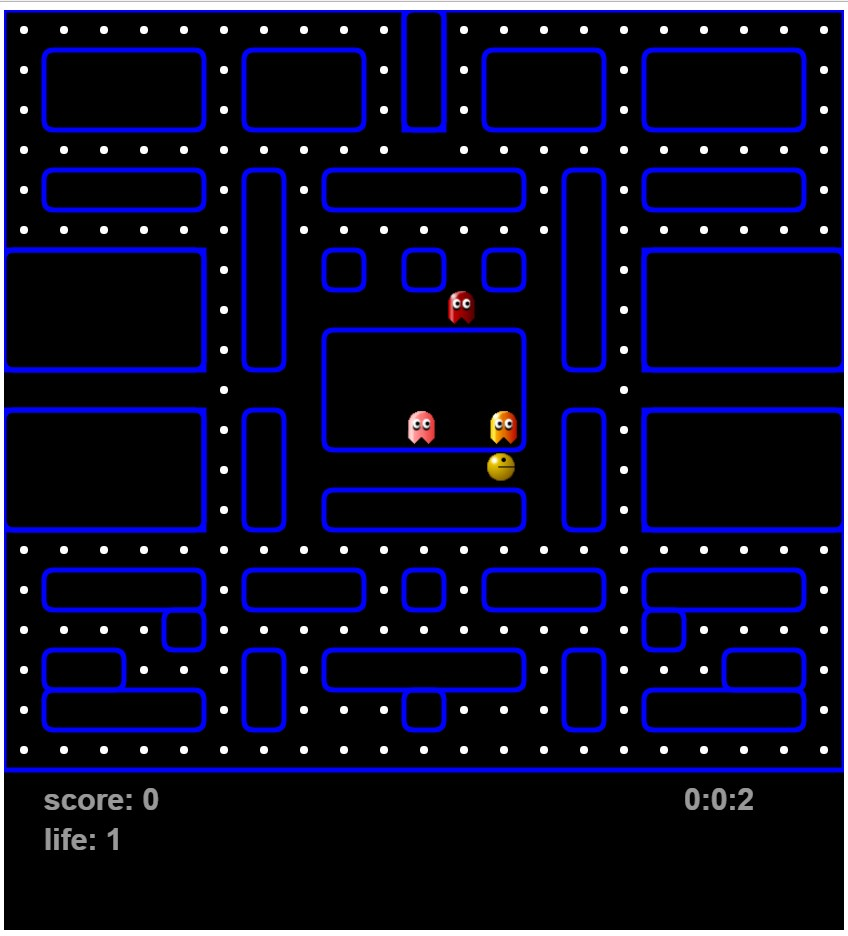
\includegraphics[width=80mm]{Figures/InitGame}
\decoRule
\caption[Inicio Juego]{Inicio juego Pacman.}
\label{fig:InitGame}
\end{figure}
Tras la interpretacion se muestra el escenario de juego con sus elementos y un panel informativo con datos de la partida \ref{fig:InitGame}.
\\Para iniciar la aplicacion el usuario pulsa la tecla 'L'  probocando el movimiento de los fantasmas y el inicio del cronometro.A partir de este momento el usuario puede manipular a Pacman a traves de las flechas del teclado ademas se permite al usuario parar el juego pulsado la tecla 'P' e iniciar nuevamente el juego con la tecla 'L' imagen\ref{fig:Pause/Start game}.
\begin{figure}[!h]
\centering
\subfigure[Juego pausado]{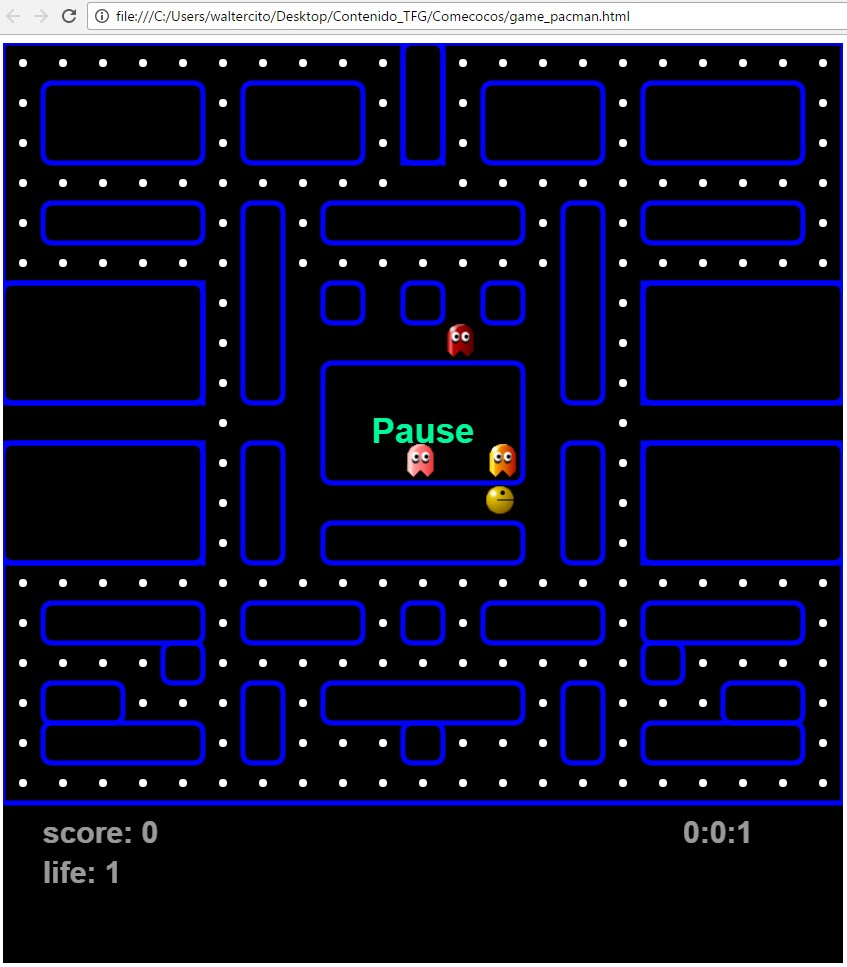
\includegraphics[width=43mm]{./PauseGame}}\hspace{5mm}
\subfigure[Juego no pausado]{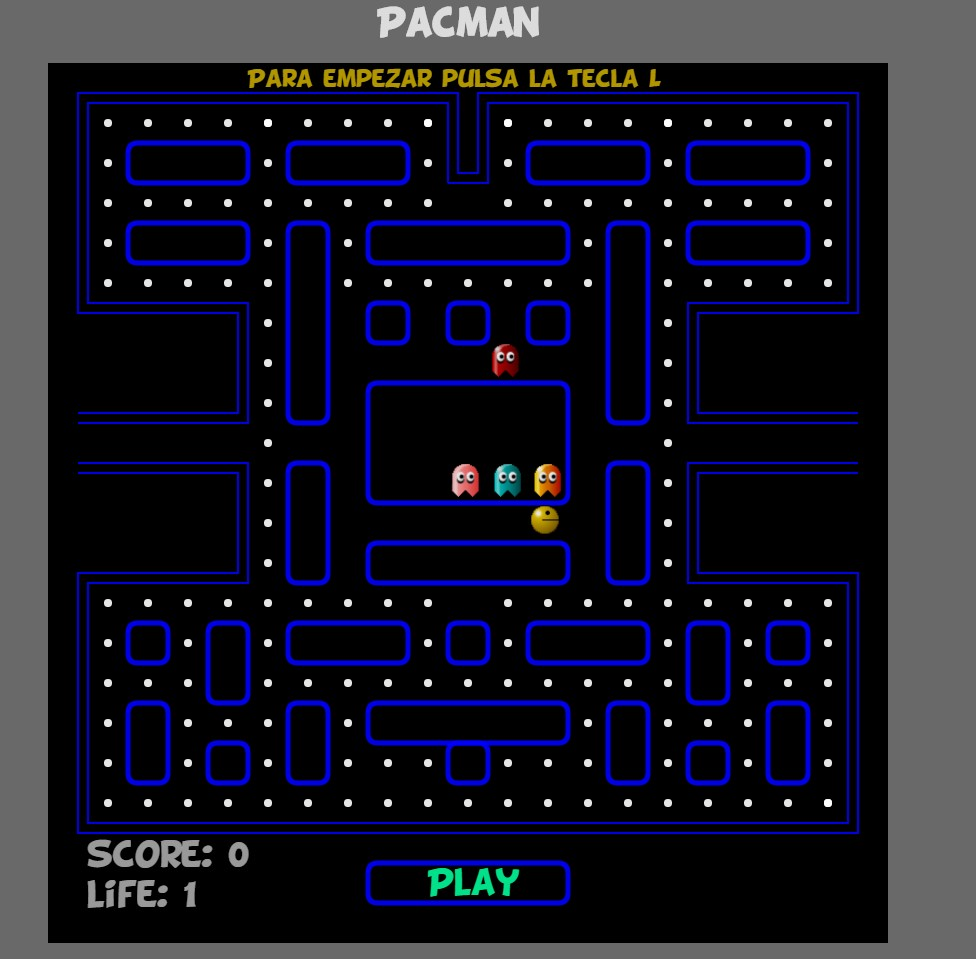
\includegraphics[width=43mm]{./InitGame}}
\caption{Pause/Start juego.} \label{fig:Pause/Start game}
\end{figure}
\\Finalmente, el juego termina cuando se produce algunas de las situciones que se mencionan a continuacion  \ref{fig:Game/Loose game}
\begin{enumerate}
\item Cuando uno de los fantasmas atrapa a Pacman daremos la partida como perdida y en la pantalla se visualiza 'Game Over'.
\item Cuando Pacman se ha comido todos los cocos la partida finaliza la partida y el usuario ha ganado la partida. El usuario visualiza 'Win Game' y si quiere guardar informacion de la partida puede pulsar 'Save Score'.
\end{enumerate}
\begin{figure}[!h]
\centering
\subfigure[Partida perdida]{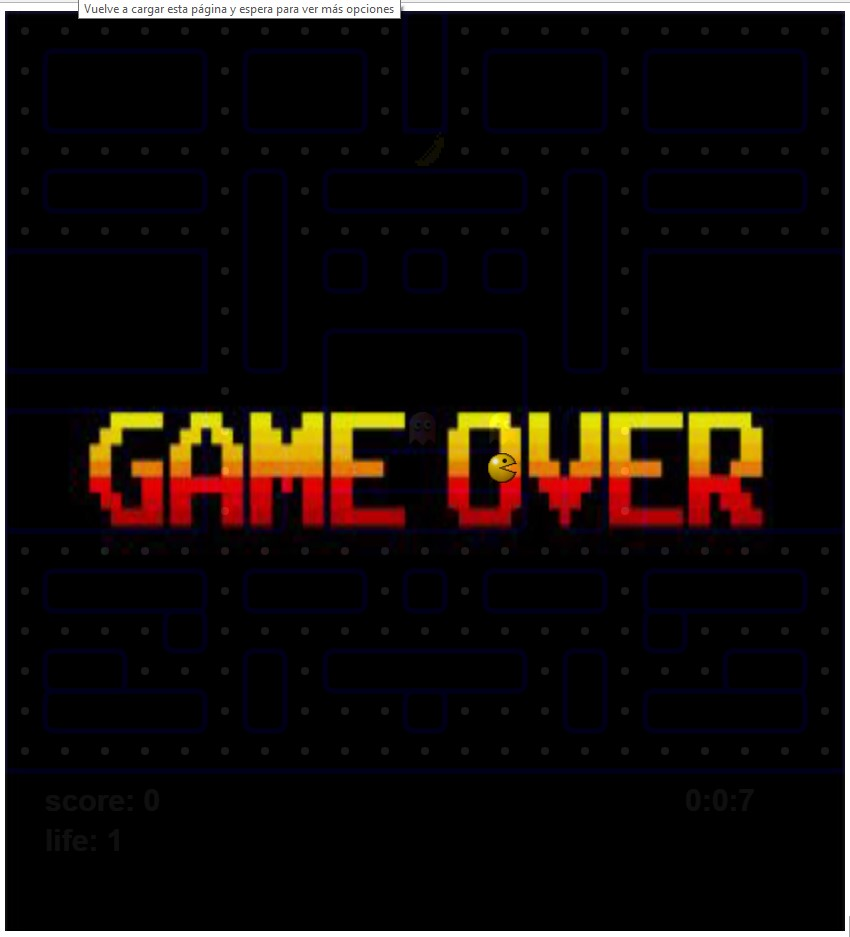
\includegraphics[width=40mm]{./GameOver}}
\subfigure[Partida Ganada]{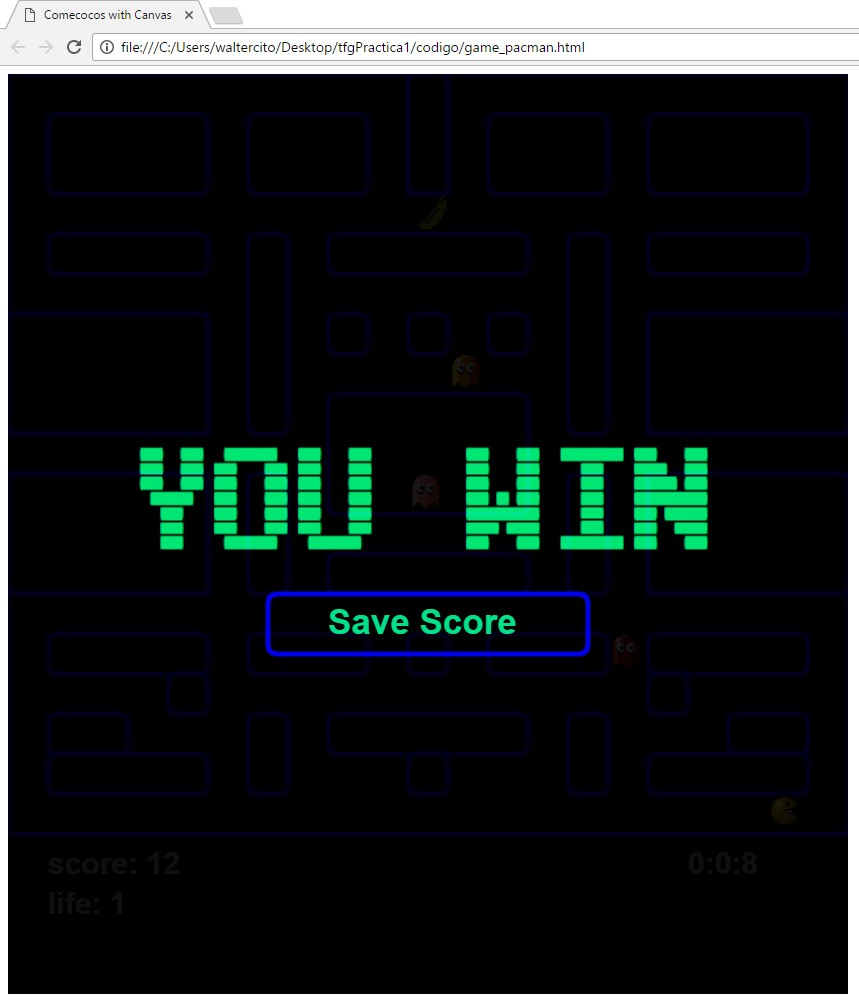
\includegraphics[width=40mm]{./Win_Game}}
\caption{Game/Loose juego.} \label{fig:Game/Loose game}
\end{figure}
